\documentclass{article}
\usepackage{graphicx,float,subcaption}
\title{Ph 21.3- Image Processing}
\author{Stella Wang}
\begin{document}
	\maketitle
\begin{enumerate}
	\item I imported an image of a chameleon in the desert 
	\begin{figure}[H]
	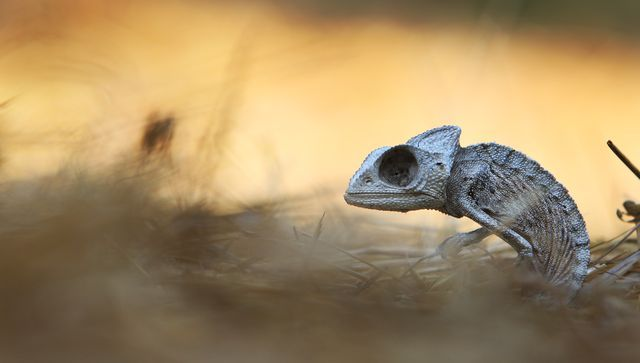
\includegraphics[width = \textwidth]{chameleon.jpeg}
	\end{figure}
	\item  
	\item Using ImageFilter.FINDEDGES, the following image was obtained. 
	\begin{figure}[H]
	\includegraphics[width= \textwidth]{FindEdges.pdf}
	\end{figure}
	\item The image was blurred using a Gaussian profile filter. 
	\begin{figure}[H]
	\includegraphics[width = \textwidth]{blur.pdf}
	\end{figure}
	\item The width parameter for the Gaussian stencil was varied from $ 0.5 to 2.0 $in the ndimage.gaussiangradientmagnitude function
	\begin{figure}[H]
	\includegraphics[width = \textwidth]{widthtest.pdf}
	\end{figure}
	\item Using different stencils, the following edge detections were obtained. The Prewitt and Sobel filters are fairly effective for edge detection and comparable to the FINDEDGES function. In order to defeat CAPTCHAS edge detection and a substantial neural net would have to be developed, but no attempted methods have worked thus far. Edge detection is also useful for image based data analysis, such as in Cell Biology.
	\begin{figure}[H]
	\begin{subfigure}{.5\textwidth}
		\centering
		\includegraphics[width = .8\linewidth]{Sobel.pdf}
		\caption{Sobel Filter}
	\end{subfigure}
	\begin{subfigure}{.5\textwidth}
		\centering
		\includegraphics[width = .8\linewidth]{Prewitt.pdf}
		\caption{Prewitt Filter}
	\end{subfigure}
	\end{figure}
	\item I learnt that there are functions that apply the gaussian gradient for you you as well as a generic derivative function that can apply numerous filters. Edge detection is important for many types of scientific research and developments in this field could prove to aid in a lot of scientific research. 
\end{enumerate}
\end{document}